\scanpage{163}
\margin{365}
(3) signifient que
\figure{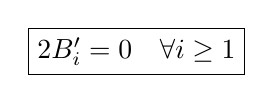
\begin{tikzpicture}\node[draw,rectangle] {$2B'_i=0\quad\forall i\geq1$};\end{tikzpicture}}
]. Il en est de même si $\varphi_*$ est un isom
($\Leftrightarrow$ \unsure{$\varphi_0$ et $\varphi_1$} un isom) car alors on voit que le coefficient dominant $a'_1$ de $\unsure{A_1|A'}(X_0)=a'_1X_0+\unsure{\mathbin{\text{---}}}$ est inversible dans $S'$.
Aussi dans les conditions du cor. 5, si $(\varphi_0(T))_{\mathrm{pd}}=(T')_{\mathrm{pd}}$ i.e.
\[
 \varphi_0(T)=\sum_{i\geq1}\lambda_i T'^{(i)}
\]
avec $\uline{\lambda_1}$ \uline{inversible}, alors \unsure{en} vertu de (2) on \unsure{trouve}
\[
 a'_1\equiv1\bmod\unsure{S_{k'}^+|S'^+}
\]
donc $a'_1$ est élément régulier \unsure{dans ce cas}.
Ainsi (3) s'écrit encore
\figure{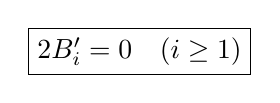
\begin{tikzpicture}\node[draw,rectangle] {$2B'_i=0\quad(i\geq1)$};\end{tikzpicture}}
\margin{$\unsure{\longrightarrow92|292}$}

\begin{center}- 47 -\end{center}\hfill IX

cette filtration induit une filtration analogue de $U(\ell)=U_\ell\otimes_{\mathbb Z_\ell}\mathbb F_\ell$, dont les facteurs successifs sont déduits des facteurs $V_i$ $(i=1,2,3)$
\[
 U^{\mathrm{et}},\quad U^{\mathrm{ef}}/U^{\mathrm{et}},\quad U/U^{\mathrm{ef}}
\]
intervenant dans la filtration (4.1.1) par tensorisation par $\mathbb F_\ell$. Bien entendu, cette filtration est stable sous $\Gamma$, et donne par additivité une décomposition de $\operatorname{long}\operatorname{Hom}_{\mathbb Z_\ell(\Gamma)}(L,U(\ell))$ en somme de trois termes, longueurs des groupes
\[
 (*)\quad\operatorname{Hom}_{\mathbb Z_\ell(\Gamma)}(L,V_i\otimes_{\mathbb Z_\ell}\mathbb F_\ell)
 \simeq(\operatorname{Hom}_{\mathbb Z_\ell(\Gamma)}(L,V_i))\otimes_{\mathbb Z_\ell}\mathbb F_\ell\ ,
\]
l'isomorphisme écrit dans (*) résultant encore de l'hypothèse de projectivité faite sur $L$ ; on suppose seulement $K'$ choisi assez grand pour que $\Gamma$ opère sur les $V_i$. Or $\operatorname{Hom}_{\mathbb Z_\ell(\Gamma)}(L,V_i)$ est évidemment un $\mathbb Z_\ell$-module sans torsion, donc son \uline{rang} est égal au deuxième membre de (*). Si $\varphi_i$ est le caractère de la représentation de $\Gamma$ dans $V_i$, et $\psi$ le caractère de la représentation de $\Gamma$ dans $\check L$, on trouve donc
\[
 \begin{aligned}
 (4.6.1)\quad\operatorname{long}\operatorname{Hom}_{\mathbb Z_\ell(\Gamma)}(L,U(\ell))
 &=\sum_{1\leq i\leq3}N^{-1}\sum_{g\in\Gamma}\psi(g)\varphi_i(g)\\
 &=N^{-1}\sum_{g\in\Gamma}\psi(g)\varphi(g),\quad\text{avec }N=\operatorname{card}\Gamma,
 \end{aligned}
\]
où $\varphi(g)=\sum\varphi_i(g)$ est aussi la fonction sur $\Gamma$ déduite par passage au quotient de la fonction sur le groupe d'inertie $I$ caractère de la représentation de monodromie de $I$ sur $U$. Or en vertu de 4.3 a) ce caractère est une fonction à \uline{valeurs entières rationnelles indépendante} de $\ell$.
Prenant $L=\mathrm{Sw}$, il en est de même du caractère $\psi(g)$ de $L$, qui est égal à $a-N\delta+1$, où $\delta$ est la ``\uline{fonction de Dirac}'' de $\Gamma$, et $a$ le ``\uline{conducteur}
\margin{162}
